\documentclass{anstrans}
%%%%%%%%%%%%%%%%%%%%%%%%%%%%%%%%%%%
\title{Residual Monte Carlo Transport in Time with Consistent Low-Order Acceleration for
    1D Thermal Radiative Transfer}
\author{Simon R.~Bolding and Jim E.~Morel}

\institute{Texas A\&M University Nuclear Engineering Department, 
}

\email{sbolding@tamu.edu \and morel@tamu.edu}

% Optional disclaimer: remove this command to hide
%\disclaimer{Notice: this manuscript is a work of fiction. Any resemblance to
%actual articles, living or dead, is purely coincidental.}

%%%% packages and definitions (optional)
\usepackage{graphicx} % allows inclusion of graphics
\usepackage{booktabs} % nice rules (thick lines) for tables
\usepackage{microtype} % improves typography for PDF
\usepackage{comment}
\usepackage{float}

\newcommand{\SN}{S$_N$}
\renewcommand{\vec}[1]{\bm{#1}} %vector is bold italic
\newcommand{\vd}{\bm{\cdot}} % slightly bold vector dot
\newcommand{\grad}{\vec{\nabla}} % gradient
\newcommand{\ud}{\mathop{}\!\mathrm{d}} % upright derivative symbol
\renewcommand{\eqref}[1]{(\ref{#1})}
\renewcommand*\thetable{\Roman{table}}
\usepackage{caption}

\captionsetup[table]{labelsep=period}
\captionsetup[figure]{labelsep=period}
\newcommand{\N}{\mathbb{N}}
\newcommand{\Z}{\mathbb{Z}}
\newcommand{\deriv}[2]{\frac{\mathrm{d} #1}{\mathrm{d} #2}}
\newcommand{\pderiv}[2]{\frac{\partial #1}{\partial #2}}
\newcommand{\bx}{\mathbf{X}}
\newcommand{\ba}{\mathbf{A}}
\newcommand{\by}{\mathbf{Y}}
\newcommand{\bj}{\mathbf{J}}
\newcommand{\bs}{\mathbf{s}}
\newcommand{\B}[1]{\ensuremath{\mathbf{#1}}}
\newcommand{\Dt}{\Delta t}
\renewcommand{\d}{\mathrm{d}}
\newcommand{\mom}[1]{\langle #1 \rangle}
\newcommand{\xl}{{x_{i-1/2}}}
\newcommand{\xr}{{x_{i+1/2}}}
\newcommand{\il}{{i-1/2}}
\newcommand{\ir}{{i+1/2}}
\newcommand{\keff}{\ensuremath{k_{\text{eff}}}}
\newcommand{\sig}[1]{\ensuremath{\Sigma_{#1}}}
\newcommand{\ra}{\ensuremath{\rightarrow}}
\newcommand{\dd}{\ensuremath{\mathrm{d}}}
\renewcommand{\O}{\ensuremath{\mathbf{\Omega}}}
\newcommand{\adj}{\ensuremath{{}^{\dagger}}}
\newcommand{\x}{\ensuremath{\mathbf{x}}}
\newcommand{\T}{\ensuremath{\text{T}}}
\newcommand{\iso}[2]{$^{#2}$#1}
\newcommand{\phibar}{\ensuremath{\overline{\phi}}}
\newcommand{\cur}[1]{\left\{ #1 \right\}}
\newcommand{\jl}{{j-1/2}}
\newcommand{\jr}{{j+1/2}}
\newcommand{\E}[1]{\ensuremath{\operatorname{E}_{#1}}}
\newcommand{\rface}{\ensuremath{r_{\text{face}}}}
\newcommand{\FOM}{\ensuremath{\text{FOM}}}
\newcommand{\ds}[0]{\displaystyle}
\newcommand{\invcm}[0]{cm$^{-1}$}
\renewcommand{\u}[1]{\ensuremath{\underline{#1}}}
\newcommand{\dep}{\ensuremath{\delta\epsilon^{(m)}}}
\renewcommand{\ss}{\ensuremath{\|s\|}}
\newcommand{\pos}{{\text{pos}}}
\newcommand{\phsp}{\ensuremath{\left(\mathbf{r},\mathbf{\Omega},\nu,t\right)}}
\newcommand{\Del}{\ensuremath{\nabla}}


\begin{document}
%%%%%%%%%%%%%%%%%%%%%%%%%%%%%%%%%%%%%%%%%%%%%%%%%%%%%%%%%%%%%%%%%%%%%%%%%%%%%%%%
\section{Introduction}

Accurate solution to the thermal radiative transfer (TRT) equations is important in the
high-energy, high-density physics regime, e.g., for inertial
confinement fusion and astrophysics simulations.  Moment-based hybrid Monte Carlo (MC)
methods have demonstrated great potential for accelerated
solutions to TRT problems.   Such methods iterate between a
high-order (HO) transport equation and a low-order (LO) system formulated with angular moments
of the transport equation over a fixed spatial mesh.  Physics operators that
are too expensive for the HO solver to resolve directly, e.g., photon absorption and emission,
are moved to the LO system. The lower-rank LO equations can be solved with Newton
methods to allow for non-linearities in the LO equations to be efficiently
resolved.  The high-order (HO) problem is defined by the transport equation
that models the photon radiation with sources defined by the previous LO solution. Solution to the HO
problem is used to construct consistency terms that require the next LO solution to be
consistent with the HO solution.  These consistency terms preserve the accuracy of the MC
solution method in the LO equations, upon nonlinear convergence of the outer iterations.

Previously, residual Monte Carlo (RMC) methods have been used to provide efficient
solution to the HO transport problem~\cite{rmc,bolding_nse}; high-fidelity solutions,
with minimal statistical noise, have been achieved for problems with optically-thick, diffusive
regions that lead to slowly varying
solutions.  However, the results in these works used a backward
Euler (BE) discretization for the time variable, which can inaccurately disperse radiation
wavefronts in optically thin problems. We have extended the work
in~\cite{bolding_nse} to include higher-accuracy treatment of the time variable for the
radiation unknowns. The exponentially-convergent Monte Carlo (ECMC)
algorithm~\cite{bolding_nse} was modified to include integration of the time variable;
this includes the introduction of a step, doubly-discontinuous (SDD) trial space representation
in time.  A new
parametric closure of the LO equations, introducing additional time-closure consistency
terms, was derived to capture the time accuracy of the HO
ECMC simulations.  The LO equations can preserve the accuracy of MC radiation transport treatment in
time, with the same numerical expense as Backward Euler (BE) time discretized S$_2$ equations. We have derived the LO equations directly from the transport equation,
such that, neglecting spatial discretization differences,
the HO and LO solutions are consistent upon convergence.
Herein we briefly describe the HO and LO solvers, and we preset results for
one-dimensional (1D), grey test problems.  We compare our method to the implicit MC
(IMC) method~\cite{wollaber_review}, the standard MC solution
method for TRT problems.

%%%%%%%%%%%%%%%%%%%%%%%%%%%%%%%%%%%%%%%%%%%%%%%%%%%%%%%%%%%%%%%%%%%%%%%%%%%%%%%%
\section{Methodology}
The 1D, grey TRT equations consist of the radiation and
material energy balance equations, i.e.,\vspace{-0.05in}
\begin{align}\label{ho_cont}
    \frac{1}{c}\pderiv{I(x,\mu,t)}{t} + \mu \pderiv{I(x,\mu,t)}{x} &+ \sigma_a
    I(x,\mu,t)
= \frac{1}{2} \sigma_a a c T^4(x,t)
    \\ \label{t_cont}
  \rho c_v \pderiv{T(x,t)}{t} &=  \sigma_a \phi(x,t) - \sigma_a a c T^4(x,t),
\end{align}
where physical scattering could optionally be included in Eq.~\eqref{ho_cont}, and
appropriate initial and boundary conditions are specified.
In the above equations $x$ is the position, $t$ is the time, $\mu$ is
the $x$-direction cosine of the angular intensity $I(x,\mu,t)$, $\sigma_a$ is the
macroscopic absorption cross section (cm$^{-1}$), and $a$, $c$, $\rho$,
and
$c_v$ are the radiation constant, speed of light, mass density, and specific heat,
respectively.  The desired transient unknowns are the material
temperature $T(x,t)$ and the mean radiation intensity $\phi(x,t)=\int_{-1}^1
I(x,\mu,t) \d \mu$.  The mean intensity is related to the radiation energy density
$E_r$ by the relation $E_r = \phi/c$.  The equations can be 
strongly coupled through the gray Planckian emission source $\sigma_a a c T^4$, which
is a nonlinear function of temperature, and the absorption
term $\sigma_a \phi$.   In general, the material properties are a function of $T$.  

In the HOLO context, the LO solver models the physical scattering and
resolves the material temperature spatial distribution $T(x)$ over each time step.  The HO solver
computes angular and temporal relations for $I$.  The
fully-discrete LO equations are based on algebraic manipulations of exact moment equations,
formed over a spatial finite-element (FE)
mesh.  The BE time discretization is applied to emission source throughout, but the radiation
variables are left in terms of time-averaged and end-of-time-step unknowns.  This is analagous to
the time-integration in IMC~\cite{wollaber_review}.   Angularly, the LO
radiation equations are similar to S$_2$ equations,  with element-averaged
consistency parameters that are weighted averages of $\mu$.  Additional
consistency parameters are introduced in a parametric closure that eliminates the auxillary
time-unknowns for radiation quantities.
If the angular and time
consistency parameters were estimated exactly, then the LO equations are exact moment equations,
neglecting spatial discretization error.  The consistency parameters are lagged
in each LO solve, estimated from the previous HO solution for $I(x,\mu,t)$,
as explained below. For the initial LO solve, within a time step, the angular parameters
are calculated based on the $I(x,\mu)$ from the previous time step and the LO equations use a standard time discretization.  The LO equations always conserve energy,
independent of the accuracy of the consistency terms.

The solution to the LO system is used to construct a spatially linear-discontinuous (LD) FE representation of
the emission source on the right hand side of Eq.~\eqref{ho_cont}.  This defines a fixed-source, pure absorber
transport problem for the HO operator. This HO transport problem represents a characteristic method that uses MC to
invert the continuous streaming plus removal operator with an LD representation of
sources. We will solve this transport problem using the ECMC algorithm.  The ECMC
algorithm is an iterative residual MC (RMC) method, which uses
batches of MC histories to estimate the error in the current trial-space representation of the
$I(x,\mu,t)$.  It is noted that because we are not using
mesh adaptation in this work, exponential convergence in iterations cannot be maintained,
but reduced variance from the RMC formulation can still be achieved.  The output from ECMC is a projection $\tilde I(x,\mu,t)$ of the intensity onto
the chosen trial space. This projection will accurately resolve the end-of-time step intensity. Once computed, $\tilde{I}(x,\mu)$ is used to directly evaluate the
necessary LO angular consistency parameters and the time closure.   The HO solution is not used to directly estimate a new temperature at
the end of the time step; it is only used to estimate the parameters that go into the LO
equations, which eliminates typical operator splitting stability issues that require linearization of
the emission source.

The process of performing subsequential HO and LO solves occurs within a single time step, can
be repeated to obtain an increasingly accurate solution for $\phi^{n+1}(x)$ and
$T^{n+1}(x)$. However, for the problems tested here, only a single HO solve is performed during each
time step.  Thus, the HOLO algorithm, for the $n$-th time step, is

\begin{enumerate}
    \item Perform a LO solve to produce an initial guess for $T_{LO}^{n+1}(x)$
        and $\phi_{LO}^{n+1}(x)$, based on consistency terms estimated with
        $\tilde{I}^{n}(x,\mu)$ and a BE time
    discretization.
\item Solve the HO system for $\tilde{I}_{HO}(x,\mu,t)$ using ECMC, based on the current
    LO estimate of the emission and scattering sources.%$\sigma_s(T^k)\phi^{k}$ and $B(T)^{k}$.
\item Compute LO consistency parameters with $\tilde{I}_{HO}^{n+1}$.  
\item Solve the LO system using HO consistency parameters to produce a new
    estimate of $\phi^{n+1}_{LO}$ and $T^{n+1}_{LO}$.
\item Store $\tilde{I}^{n}\leftarrow\tilde{I}^{n+1}$, and move to the next time step.
\end{enumerate}

\subsection*{The LO System}
\label{sec:lo}

To derive the LO equations, we reduce the dimensionality of Eq.~\eqref{ho_cont} and
Eq.~\eqref{t_cont} by taking spatial, angular, and
temporal integrals.  The spatial moments are taken over each spatial cell $i$:
$x\in[x_{i-1/2},x_{i+1/2}]$, weighted with the standard linear Lagrange interpolatory FE basis functions.  For example, the left moment operator is defined by
\begin{equation}\label{x_mom}
    \mom{\cdot}_{L,i} = \frac{2}{h_i} \int_{x_{i-1/2}}^{\xr} b_{L,i}(x) (\cdot) \d x,
\end{equation}
where $h_i=x_{i+1/2}-x_{i-1/2}$ is the width of the spatial element and
$b_{L,i}(x)=(x_{i+1/2}-x)/h_i$ is the basis function corresponding to position
$x_{i-1/2}$. Angularly, the equations are integrated over the positive and negative half
ranges.  The angular integrals of the intensity are defined as $\phi^\pm(x) = \pm2\pi
\int_0^{\pm 1} \psi(x,\mu) \d \mu$.  Finally, the equations are integrated over the $n$'th
time step defined for 
$t\in[t^n,t^{n+1}]$ with width $\Delta t = t^{n+1}-t^{n}$.  

The positive half-range integral, $\mom{\cdot}_{L,i}$ moment, and
integration over a time step of Eq.~\eqref{ho_cont} yields
\begin{multline}\label{eq:t_moml_ex}
    \frac{\mom{\phi}_{L,i}^{+,n+1} - \mom{\phi}_{L,i}^{+,n}}{c \Delta t}
    -2\overline {\mu}_{i-1/2}^{\,+} \overline \phi_{i-1/2}^{\,+} + \overline{\cur {\mu}}_{L,i}^{+}
  \mom{\phibar}_{L,i}^{+}
  +  \overline{\cur\mu}_{R,i}^{+}
  \mom{\phibar}_{R,i}^{+} \\ +  \sigma_{a,i}^{n+1} h_i 
  \mom{\overline\phi}_{L,i}^{n+1,+}   = \frac{h_i}{2} \mom{\sigma_a^{n+1} a c T^{n+1,4}}_{L,i},
\end{multline}
where overlined quantities denote time averaging.  The time-averaged angular consistency
terms are approximated with the previous HO solution, e.g.,
\begin{equation}\label{const}
    \overline{\cur{{\mu}}}_{L,i}^+ =  \frac{
        {\displaystyle \frac{2}{h_i}} \int\limits_0^1 \int\limits_\xl^\xr \mu \, b_{L,i}(x)
        \overline{I}(x,\mu) \d x \d \mu } 
{{\displaystyle \frac{2}{h_i}} \int\limits_0^1 \int\limits_\xl^\xr \, b_{L,i}(x)
\overline{I}(x,\mu) \d x \d \mu } .
\end{equation}
where $\overline{I}(x,\mu)$ is a time-averaged LDFE projection in $x$ and $\mu$, as
explained in the next section.  For simplicity, the face terms are eliminated from the system using a LDFE
spatial approximation, with upwinding.  There is some inconsistency introduced in this approximation, but
it has proven stable for problems tested and demonstrates preservation of the equilibrium diffusion
limit~\cite{morel_ldtrt}.

The LO equations must now be closed in time consistently with the HO
equations.   Previous work has enforced
consistency in time by adding a local artificial source to the time-discretized LO
equations in each cell~\cite{holo_rh}.  This
source was approximated based on the difference between the exact HO integral of the time
derivative and the approximate BE representation in LO equations. We will alternatively use a
parametric closure for the radiation unknowns. 

Quantities at $t^{n}$ are known from the previous time step or an initial condition.  
So Eq.~\eqref{eq:t_moml_ex} can be written exclusively in terms
of time-averaged radiation unknowns, if $\mom{\phi}_{L,i}^{n+1}$ is eliminated from the
system.  The simplest closure is a weighted average
\begin{equation}
    \mom{\phi}_{L,i}^{+,n+1} \simeq \gamma_{L,i,HO}^+ \mom{\phi}_{L,i}^+
\end{equation}
where $\gamma_{L,i,HO}^+$ is a time-closure consistency parameter.  The previous HO solution to the
above equation provides the value for the consistency parameter.  For the first solve
during a time step, all $\gamma$ values are set to unity, producing a BE discretization.
but other closures, such as a modified Crank-Nicolson have been explored.  In optically
thin problems, the problem is nearly linear, and the choice of this closure becomes
relatively arbitrary since all other unknowns have been eliminated from the system.
Once the time-averaged unknowns have been calculated,
the local time closures can be used to convert the time-averaged unknowns to end-of-time-step
values.  There are four time-closure consistency parameters, for each LO element. 

The other equations can be derived analogously.  More specifics on the angular and spatial
manipulation of equations can be found in literature~\cite{wolters,bolding_nse}.  
Summing the equations over all cells, a global, nonlinear LO system of equations is formed
for the moment unknowns.  This system of equations is solved using an analytic Newtons method, as in
previous work~\cite{bolding_nse}.  We have also investigated the use of source iteration
with an approximate diffusion synthetic acceleration method~\cite{wsa} to invert the scattering
operator within Newton iterations~\cite{wla}. 

\subsection*{The Residual MC High Order Solver}
\label{sec:ho}

The transport equation to be solved by ECMC is given by Eq.~\eqref{ho_trans}, but with a
known LDFE Planckian emission source:
\begin{equation}\label{te_oper}
    \B L I(x,\mu,t)  = q_{LO}(x)
\end{equation}
where $q_{LO}$ denotes the latest estimate of the isotropic emission source, using $T_{LO}^{n+1}(x)$.  The \emph{continuous} linear operator $\B L$ includes the streaming, removal, and
time derivative on the left-hand side of Eq.~\eqref{ho_trans}.  

To apply the residual MC algorithm, it is necessary to have a trial space representation
of the solution for all phase space variables.  The intensity is represented in $x$ and $\mu$ with a
LDFE projection~\cite{bolding_nse}.  This projection preserves the zeroth, and
first moment in $x$ and $\mu$, over each space-angle cell.  A step, doubly-discontinuous (SDD) trial
space is used to represent the intensity as a function of $t$.  The trial space
representation for $I(x,\mu,t)$ is then
\begin{equation}\label{eq:time_space}
    \tilde I(x,\mu,t) = \left \{ \begin{array}{cl}
        \tilde I^{n}(x,\mu)  & \quad t = t^n \\ 
        \overline I(x,\mu)  & \quad t^{n} < t <t^{n+1} \\               
      \tilde I^{n+1}(x,\mu)   &  \quad        t = t^{n+1}
    \end{array}           \right.
\end{equation}
where we have used $\overline I$ to denote the time-averaged LDFE \emph{projection} in $x$
and $\mu$ of the intensity over the interior of the time step;  the LDFE projections at
$t^{n}$ and $t^{n+1}$ are denoted $\tilde I^{n}$ and $\tilde I^{n+1}$, respectively.    
 The SDD trial space provides a
projection for all the desired unknowns that result from time-integration of the transport
equation to produce a balance equation, i.e., the time-averaged, end of time step, and
previous time step intensities. Another benefit of this
trial space is it allows for infrastructure for sampling from residual from the
time-discrete formulation to be used directly. A drawback of the RMC approach is that
a truncation error occurs by keeping only the LDFE projection of the intensity between
time steps.  Adaptive mesh refinement is likely necessary to capture highly-peaked solutions, but
this could be included in the iterative ECMC algorithm.

To define the ECMC algorithm, we note that $q_{LO}$ remains constant over the entire HO solve.
The $m$-th approximate solution to Eq.~\eqref{te_oper} is $\tilde{I}^{(m)}$, where
$m$ identifies the MC batch.
The $m$-th residual is $r^{(m)} = q - \B L\tilde{I}^{(m)}$, which with manipulation gives the error equation
\begin{equation}
\B L (I - \tilde{I}^{(m)}) = \B L {\epsilon}^{(m)} = r^{(m)}
\end{equation}
where $I$ is the exact solution (for the problem which includes projection error of the
previous time step) and $\tilde{\epsilon}^{(m)}$ is finite element
representation, in space and angle, of the error in
$\tilde{\psi}^{(m)}$. The above equation represents an auxiliary, fixed-source, pure
absorber transport equation.
The operator $\B L$ is inverted without discretization via MC simulation to produce an
estimate of the error in $\tilde{\psi}^{(m)}$, i.e., $\tilde{\epsilon}^{(m)} = \B
L^{-1} r^{(m)}$.  The MC simulation samples particles from the source $r^{(m)}$, which
produces negative and positive weights.  Histories are tracked in space, angle, and time, as for IMC~\cite{wollaber_review}.
The LDFE projection $\overline{\epsilon}$ is computed using generalized volumetric path-length estimators. 
A generalization of tallies used to estimate volume-averaged census energy
from IMC~\cite{wollaber_review} is used to capture the LDFE projection
$\epsilon^{n+1}(x,\mu)$.  The estimators are weighted by appropriate basis
functions to tally the zeroth and first moments, in $x$ and $\mu$, of $I(x,\mu)$ over each
space-angle cell.  

Sampling from the residual is extended to the time variable from previous work.  It is
noted that the discontinuities in the trial space introduce $\delta$-function sources
because of $\pderiv{\tilde{I}}{t}$.  
However, the contribution from the discontinuity source at $t^{n+1}$ can be analytically
estimated such that it does not need to be sampled; the result is that $\tilde I^{n+1}$ is
error particles that reach the time step and $\overline I^{(m)}(x,\mu)$.  

  The ECMC algorithm is
\begin{enumerate}
\item Solve Eq.~\eqref{te_oper} to compute the MC projection of the angular
flux onto the LD $x-\mu$ trial space $\tilde\psi^{(0)}$.
\item Compute $r^{(m)}$.
\item Estimate $\tilde{\epsilon}^{(m)} = \B L^{-1} r^{(m)}$ with $N$ Monte Carlo histories.
\item Compute $\tilde I^{(m+1)} = \tilde I^{(m)}
+ \tilde\epsilon^{(m)}$
\item Optionally repeat 2 -- 4 for desired number of batches.
\end{enumerate}


%%%%%%%%%%%%%%%%%%%%%%%%%%%%%%%%%%%%%%%%%%%%%%%%%%%%%%%%%%%%%%%%%%%%%%%%%%%%%%%%
\section*{Results and Analysis}

We have simulated two 1D, grey test problems to demonstrate the efficacy of our HOLO
algorithm: an optically thin problem and a standard Marshak wave. 
We use the L$_2$ measure of variance in the end of time step intensities to
form a figure of merit as

\subsection{Optically Thin Problem}

For this problem, material properties
are uniform throughout a 2.0 cm wide domain with $\rho c_v = 0.01374$ GJ cm$^{-3}$
keV$^{-1}$, and $\sigma_a=0.2$ \invcm.  
The material and radiation are initially in equilibrium at an effective temperature of $0.01$ keV.
An isotropic incident intensity with $T_r = 0.150$ keV is applied
at $x=0$ for $t>0$; the incident intensity on the right boundary is $0.01$ keV.
 Solutions are plotted as an effective radiation temperature
 $T_r=\left(\phi/(ac)\right)^{0.25}$ are plotted; the values for $T_r^{n+1}$ from the last
 time step are compared for IMC, HOLO method with continuous time treatment (HOLO-TC), and
 the HOLO method with full BE time discretization (HOLO-BE) in
Fig.~\ref{fig:thin_temp_compare}.  The HOLO-TC and HOLO-BE results were generated with 30
$\mu$ cells, and all spatial meshes used 200 cells.  At smaller time step sizes, the
effects of projecting the solution become apparent in the HOLO-TC results, leading to more
dispersion near the wave-front.  For $\Delta t=0.005$ sh, there is good agreement between
the HOLO-TC results and IMC.  The HOLO-BE results do not accurately capture
the wavefront location. IMC demonstrates substantial statistical noise in the equilibrium region.

\begin{figure}[H]
  \centering
    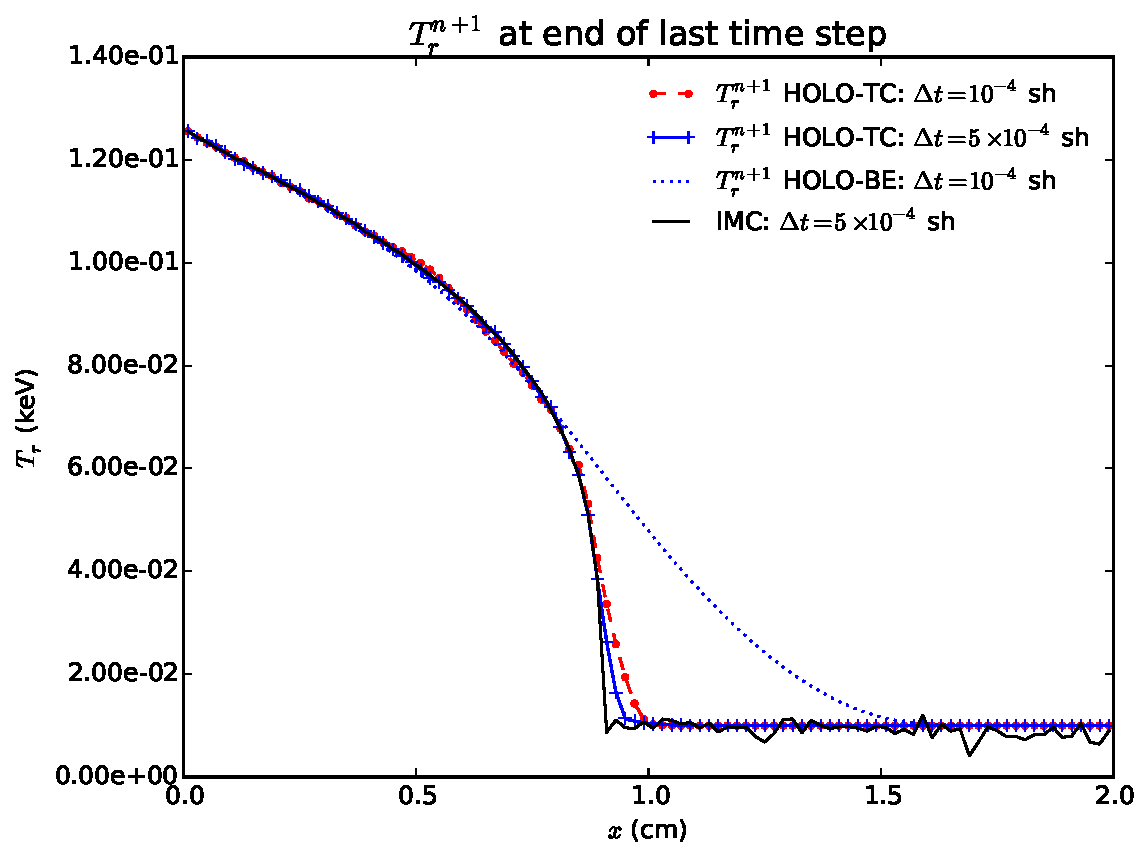
\includegraphics[width=\linewidth]{thin_temp_compare.pdf}
    \caption{\label{fig:thin_temp_compare} Comparison of radiation temperatures of IMC and
    the HOLO method for different time step sizes and numbers of batches, for optically
thin problem. }
\end{figure}

Table.~\ref{tab:fom_thin} compares computed FOM values for the census
radiation energy densities, for the case of $\Delta t =
0.0005$~sh.  HOLO results were generated for the case of 1 and 2 batches, with the same
total number of histories per time step.  At low particle counts for the larger time step
size, the HOLO-TC method
demonstrates substantial noise.  This is due to the trial space representation of the
census particles at the end of the time step being poorly estimated.  For the 2 batch
case, the estimate from the first batch leads to less error in the census estimate as the
ECMC solves are simply solving for the deviation from the time-averaged quantity.  The
results for the case of 30,000 histories are plotted in Fig.~\ref{} for the HO and LO
solution.  As demonstrated, there seems to have been some instabilities introduced into
the LO equations through noise; sufficient sampling of the census must occur.
At smaller time-steps there is an increase in statistical efficiency, however there has
been a loss in accuracy due to an increase in projection error.  In general, this is a
balance that much be considered.

The accuracy of the HOLO-ECMC method was compared to a reference solution from IMC. This
problem is thin enough that we expect IMC to be accuracy with sufficient particle
histories.  The
reference solution is the average of 20 IMC simulations of $20\times10^6$
histories, each with $\delta t =10^{-4}$ sh.  The estimated value of $\ss$ for the
reference solution is 0.025\%.  The L$_2$ norm of the error in cell-averaged mean
intensities is computed 
at the end of the last time step, was computed.  The average over 20 simulations is then
computed to provide the metric
\begin{equation}
    \|e\|^l = \left({\frac{\sum\limits_{i=1}^{N_c}
    \left(\phi_i^{n+1,l} - \phi_i^{n+1,ref}
\right)^2}{\sum\limits_{i=1}^{N_c}\left(\phi_i^{n+1,ref}\right)^2}}\right)^{1/2},
\end{equation}
where $\phi_i^{n+1,l}$ is the cell-averaged scalar intensity at the end of the last time
step from the $l$-th independent simulation.  The sample mean of $\|e\|$ from 20
independent simulations provides a metric for the accuracy of a particular simulation:
\begin{equation}
    \overline{\|e\|} = \frac{1}{20}\sum_{l=1}^{20} \|e\|^l
\end{equation}

The accuracy results for 

\begin{table}[H]
\centering
\caption{\label{tab:void_short} {Comparison of sample statistics for the
    end of time step radiation energy densities, of the last time step, for the optically
    thin problem and $\Delta t = 5\times 10^{-4}$ sh.   Simulation end time is $\mathbf{t=0.003}$ sh.}}
\vspace{-0.1in}
\begin{tabular}{|c|ccc|ccc|}\cline{2-7}
    \multicolumn{1}{c|}{}       & \multicolumn{3}{|c|}{\ss} &
    \multicolumn{3}{|c|}{\FOM} \\ \hline
hists./step   & IMC & HOLO-TC (1) & HOLO-TC (3) &  IMC   & HOLO-TC(1) & HOLO-TC(3) \\ \hline
   30,000     & 3.01\%  & 18.29\% & 5.38\%      &  1.00  & 0.03  &  0.31      \\
  300,000     & 0.99\%  & 0.81\%  & 0.74\%      &  0.93  & 1.38  &  1.65     \\ 
  1,000,000   & 0.50\%  & 0.30\%  & 0.37\%      &  1.10  & 3.42  &  2.0      \\ \hline
\end{tabular}
\end{table}

\begin{table}[H]
\centering
\caption{\label{tab:void_short} {Comparison of sample statistics for the
    end of time step radiation energy densities, of the last time step, for the optically
    thin problem and $\Delta t = 1\times 10^{-4}$ sh.   Simulation end time is $\mathbf{t=0.003}$ sh.}}
\vspace{-0.1in}
\begin{tabular}{|c|ccc|ccc|}\cline{2-7}
    \multicolumn{1}{c|}{}       & \multicolumn{3}{|c|}{\ss} &
    \multicolumn{3}{|c|}{\FOM} \\ \hline
hists./step   & IMC & HOLO-TC (1) & HOLO-TC (3) &  IMC   & HOLO-TC(1) & HOLO-TC(3) \\ \hline
   30,000     & 3.00\%  & 0.55\% & 1.28\%       &  1.00  &  29.81    & 5.51    \\
  300,000     & 0.96\%  & 0.11\% & 0.30\%       &  0.98  &  71.82    & 9.88    \\ 
  1,000,000   & 0.49\%  & 0.06\% & 0.17\%       &  1.11  &  71.02    & 9.71    \\ \hline
\end{tabular}
\end{table}


\subsection{Marshak Wave Problem}

It is important to demonstrate that the time closures are stable in a mix of optically
thick and optically thin regions, and that the ECMC method is still efficient in such
problems.  Simulations were performed for the Marshak wave problem defined in
Sec.~\ref{sec:marshak}.  The time step size is linearly increased from $0.001$ sh to a
maximum step of 0.01 sh over the first 10 time steps; the last time step is adjusted to
reach the desired simulation end time.  It was found for this problem that it was
necessary to use more than one batch for the HOLO-TC algorithm to stably converge.
This is because in the case of a single batch particles must reach
census to accurately estimate the next time step value.  These results were generated using the implicit-like time
closure.

\begin{figure}[H]
    \centering
    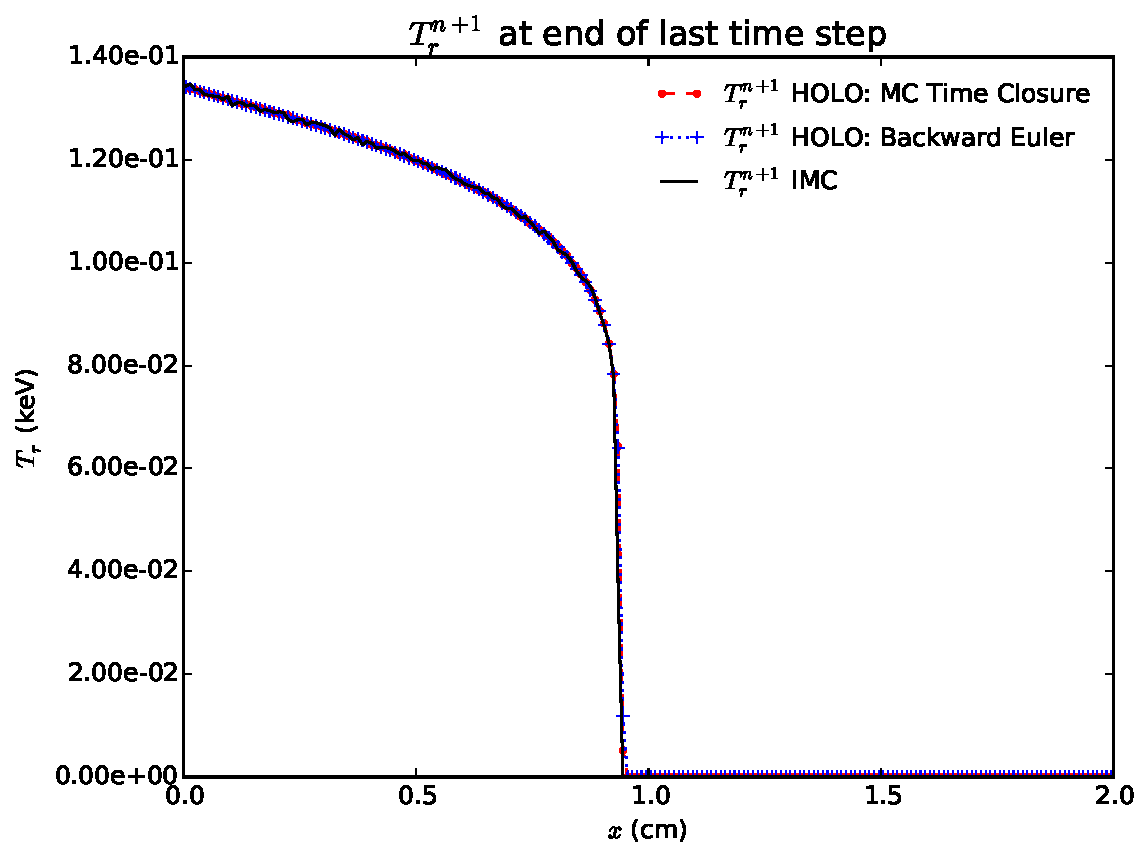
\includegraphics[width=\linewidth]{marshak_time_cont_compare.pdf}
    \caption{\label{fig:marshak_tc} Comparison of HOLO-TC, HOLO-BE, and IMC methods for
the Marshak Wave problem, with $10^6$ histories per time step.}
\end{figure}

Figure~\ref{fig:marshak_tc} compares the accuracy of IMC, HOLO-TC, and HOLO-BE.  The
solutions are plotted at $t=3$ sh, with $10^6$ histories per time step for all
simulations. As demonstrated, there is good agreement among the results.  It is noted that
this problem can be accurately modeled with the Backward Euler time discretization, but
the MC time closure appears to be stable even in the mix of optically thick and thin
regions. Table~\ref{tab:marshak_cont} compares sample statistics for IMC and
the HOLO method with continuous time treatment and with a BE discretization.  As
demonstrated, at the lower history count (300,000), the HOLO-TC algorithm demostrates a
greater variance.  These results used the implicit
like time closure.

\begin{table}[H]
\centering
\caption{\label{tab:marshak_cont} {Comparison of sample statistics for the
    end of time step radiation energy densities, of the last time step, for the marshak
    wave problem and maximum time step of $0.01$ sh.  Simulation end time is $\mathbf{t=3.0}$ sh.}}
\vspace{-0.1in}
\begin{tabular}{|c|ccc|ccc|}\cline{2-7}
    \multicolumn{1}{c|}{}       & \multicolumn{3}{|c|}{\ss} &
    \multicolumn{3}{|c|}{\FOM} \\ \hline
hists./step   & IMC & HOLO-TC (2) & HOLO-BE (2) &  IMC   & HOLO-TC (2) & HOLO-BE (2) \\ \hline
  300,000     & 2.25\%  & 3.42\% & 0.30\%       &  1.00  &   0.43    & 2050          \\  
  1,000,000   & 1.27\%  & 0.31\% & 0.17\%       &  0.94  &  15.95    & 1806          \\ \hline
  \multicolumn{7}{|c|}{Diamond Like Closure} \\ \hline
  300,000     & --  & 3.53\% & --   &  --  &   0.41   & --  \\  
  1,000,000   & --  & 0.37\% & --   &  --  &  10.94   & --  \\ \hline
\end{tabular}
\end{table}




Later on, we can include a table, even one that spans two columns such as
Table~\ref{tab:widetable}.
%%%%%%%%%%%%%%%%%%%%%%%%%%%%%%%%%%%%%%%%
\begin{table*}[htb]
  \centering
\begin{tabular}{llllllllll}\toprule
      & $\phi_T(0)$      & $\phi_T(10)$      & $\phi_T(20)$      &
      $\phi_D(0)$      & $\phi_D(10)$      & $\phi_D(20)$      & $\rho$      &
      $\varepsilon$      & $N_\text{it}$
\\ \midrule
$c=0.999$  & 0.9038 & 20.63 & 31.24 & 0.9087 & 20.63 & 31.23 & 0.2192 & $10^{-7}$ & 15
\\
$c=0.990$  & 0.3675 & 13.04 & 24.7 & 0.3696 & 13.04 & 24.69 & 0.2184 & $10^{-7}$ & 15
\\
$c=0.900$  & 0.009909 & 4.776 & 17.64 & 0.009984 & 4.786 & 17.63 & 0.2118 & $10^{-7}$ & 14
\\
$c=0.500$  & $6.069\times 10^{-5}$ & 2.212 & 15.53 & 6.213$\times 10^{-5}$ & 2.239 & 15.53 & 0.2068 & $10^{-7}$ & 13
\\
\bottomrule
\end{tabular}
  \caption{This is an example of a really wide table which might not normally
  fit in the document.}
  \label{tab:widetable}
\end{table*}


%%%%%%%%%%%%%%%%%%%%%%%%%%%%%%%%%%%%%%%%%%%%%%%%%%%%%%%%%%%%%%%%%%%%%%%%%%%%%%%%
\section{Conclusions}

Initial results demonstrate that residual MC methods can be extended to include the time
variable.  Our ECMC algorithm can be more statistically efficient than IMC, although a
high mesh resolution is needed between time steps; adaptive mesh refinement would be
highly beneficial for realistic applications.  We have demonstrated a new approach to
closing the LO equations that produces consistent solutions.  Long-term, an alternative approach would be
to operator split the census radiation.

At this point, we believe that the SDD trial space in time suffers from the fact that particles must
reach the end-of-time step to contribute to the intensity, and ultimately the closure.  Alternatively, the LDFE trial space
could also include the time variable (i.e., it is linear in time).  This has the added
benefit that the slope can be estimated over the interior of the time-step, so all
particle tracks contribute to the score.  However, there is some additional truncation
error as the end of time-step is an extrapolated quantity.  We are investigating the use
of the LD trial space, but it requires substantial modifications to the residual sampling
algorithm because analytic L$_1$ integrals of the local residuals become untenable.  An
importance sampling methodology has been developed but remains to be implemented.  Additionally, modifications to the sampling
algorithm are necessary to extend to higher spatial dimensions or polynomial order, so determining if our
approach is efficient will be of benefit to future work. We plan to include results
for the LD representation in time for the full paper. 

%%%%%%%%%%%%%%%%%%%%%%%%%%%%%%%%%%%%%%%%%%%%%%%%%%%%%%%%%%%%%%%%%%%%%%%%%%%%%%%%
\section{Acknowledgments}



%%%%%%%%%%%%%%%%%%%%%%%%%%%%%%%%%%%%%%%%%%%%%%%%%%%%%%%%%%%%%%%%%%%%%%%%%%%%%%%%
\bibliographystyle{ans}
\bibliography{references}
\end{document}

